\documentclass[serif, 12pt]{beamer}
\usepackage[utf8x]{inputenc} 
\usepackage[russian]{babel}  
\usepackage{ucs}
\usepackage{tikzsymbols}
 \usepackage{fontawesome}
 
 \usepackage{caption}
 
\usepackage{xcolor}
 
 \usepackage{mathrsfs}
 \usepackage{stackrel}
 

\usepackage[math]{kurier}
\usepackage[T1]{fontenc}
\usetheme{Madrid} 
  \useoutertheme{shadow} 
  \setbeamertemplate{bibliography item}{\insertbiblabel}
  
  
  
  \usepackage{hyperref}

  

\setbeamertemplate{footline}[page number]


\setbeamertemplate{navigation symbols}{}

\usecolortheme[named=violet]{structure}
 
 \title{Dynamics and Multivalued Groups}
\author{Mikhail Kornev} 

 \institute{Steklov Mathematical Institute of RAS
$\;$\\
$\;$\\
$\;$\\
SIMC Youth Race\\
March 13-17, 2023} 
  
  
\date{}

\usepackage{amsthm, amsmath, amssymb} % Mathematical typesetting
\usepackage{hyperref} % For hyperlinks in the PDF

\renewcommand{\qedsymbol}{\textcolor{violet}{\openbox}}

\usepackage{esint}

\newtheorem{thm}{Theorem}
\newtheorem{statement}{Statement}
\newtheorem{lemm}{Lemma}
\newtheorem{nproblem}{Problem}
\newtheorem{coroll}{Corollary}
\newtheorem{comment}{Remark}
\newtheorem{prop}{Proposition}

\theoremstyle{definition}
\newtheorem{defi}{Definition}




\DeclareMathOperator{\pp}{\mathbb{P}}
\DeclareMathOperator{\Ho}{\mathrm{Ho}}
\DeclareMathOperator{\Hig}{\mathrm{Hig}}
\DeclareMathOperator{\B}{\mathbb{B}\!}
\DeclareMathOperator{\Ll}{\mathcal{F}}
\DeclareMathOperator{\Oo}{\mathcal{O}}

\let\phi\varphi
\let\epsilon\varepsilon

\newcommand\pto{\mathrel{\ooalign{\hfil$\mapstochar$\hfil\cr$\to$\cr}}}

\usepackage{bm}

  
  
  
  
\setbeamercolor{emph}{fg=magenta}
\renewcommand<>{\emph}[1]{%
  {\usebeamercolor[fg]{emph}\only#2{\itshape}#1}%
}


\usepackage{euscript}

\begin{document}

\maketitle










\begin{frame}{Introduction}

\begin{itemize}

\item In different areas of research, multivalued products on spaces appear

\item The literature on multivalued groups and their applications is large and includes articles since XIX century mostly in the context of hypergroups

\item In 1971, S. P. Novikov and V. M. Buchstaber gave the construction, predicted by characteristic classes. This construction describes a multiplication, with a product of any pair of elements being a non-ordered multiset of $n$ points


\end{itemize}

\end{frame}













\begin{frame}{Introduction}

\begin{itemize}


\item It led to the notion of $n$-valued groups which was given axiomatically and developed by V. M. Buchstaber 

\item At present, a number of authors are developing $n$-valued (finite, discrete, topological or algebra geometric) group theory together with applications in various areas of Mathematics and Mathematical Physics

\end{itemize}

\end{frame}



















\begin{frame}{Introduction}

\begin{itemize}

\item Since 1996, V. M. Buchstaber and A. P. Veselov and became develop some applications of $n$-valued group theory to discrete dynamical systems

\item In 2010, V. Dragović showed the associativity equation for 2-valued group explains the Kovalevskaya top integrability mechanism   

\end{itemize}

\end{frame}







\begin{frame}{Introduction}

We will talk about

\begin{itemize}

\item Symbolic Dynamics

\item Tiling theory

\item Multivalued Group theory

\item their connections and some author's results  

\end{itemize}

\end{frame}


















\begin{frame}{Combinatorics on Words Preliminaries}

\begin{itemize}

\item \emph{Alphabet} $A$ is a finite set, consisting of letters 

\item $A^\ast$ stands for the \emph{monoid of finite words} in an alphabet $A$

\item $A^\omega$ stands for the set of \emph{right infinite words}

\item A word $w\in A^\omega$ is \emph{periodic} if it is of the form $w = uvvv...$ for some $u, v\in A^\ast$ 

\item A word $w\in A^\omega$ is \emph{aperiodic} (or, \emph{quasi-periodic}) if it is not periodic

\item \emph{Factor} is a finite continuous subword $u$ in $w = ...u...$

\item Denote by $|w|$ the length of a word $w\in A^\ast$

\end{itemize}


\end{frame}

















\begin{frame}{Combinatorics on Words Preliminaries}

\begin{itemize}

\item Let $A$ and $B$ be alhabets. A \emph{morphism} is a map $\Ll: A^\ast\to B^\ast$ satisfying $$\Ll(xy) = \Ll(x)\Ll(y)$$ for all words $x, y\in A^\ast$, i. e., $\mathcal{F}$ is a homomorphism of monoids

\item A morphism is defined by the images $\Ll(a)$ of the letters $a\in A$

\end{itemize}

\end{frame}












\begin{frame}{Combinatorics on Words Preliminaries}

\begin{itemize}

\item In some cases, one can define a limit $$a\to \Ll(a)\to \Ll(\Ll(a))\to ... \to \Ll^\infty(a)$$

\item It is easy to see that the word $w = \Ll^\infty(a)$ will be \emph{a fixed point}, i. e., $\Ll(w) = w$

\end{itemize}



\end{frame}














\begin{frame}{Examples of Morphisms}

\begin{block}{Example (Fibonacci Morphism)}
$$\Ll: \{0, 1\}^\ast\to \{0, 1\}^\ast, \ 0\mapsto 01,\ 1\mapsto 0$$
The \emph{infinite Fibonacci word} $\Phi := \Ll^\infty(0)$ is

$$\Phi = 01001010010010100101001001010010...$$

%01001010010010100101001001010010010100101001001010010...

\end{block}

\end{frame}













\begin{frame}{Examples of Morphisms}

\begin{block}{Example (Thue-Morse Morphism)}

$$\Ll: \{0, 1\}^\ast\to \{0, 1\}^\ast, \ 0\mapsto 01,\ 1\mapsto 10$$
The \emph{Thue-Morse sequence} $\Ll^\infty(0)$ is 

$$T = 01101001100101101001011001101001...$$
\end{block}

\end{frame}















\begin{frame}{Examples of Morphisms}

\begin{block}{Example (Tribonacci Morphism)}
$\Ll: \{a, b, c\}^\ast\to \{a, b, c\}^\ast$
$$\Ll:\begin{cases}
a\mapsto abc,\\
b\mapsto ac,\\
c\mapsto b
\end{cases}$$

The \emph{infinite tribonacci word} $\Ll^\infty(a)$ is

$$abcacbabcbacabcacbacabcb...$$


\end{block}


\end{frame}












\begin{frame}{The Factor Complexity}

\begin{itemize}

\item The \emph{factor complexity} of an infinity word $w$ is the function $f_w(n)$ defined as the number of its factors of length $n$   

\item One can show that for an infinite word $w$ there exists $C\in \mathbb{N}$ such that $$f_w(n)\leqslant C$$ for evey $n\in \mathbb{N}$ 

\end{itemize}


\end{frame}















\begin{frame}{The Factor Complexity}

\begin{thm}[M. Morse and G. Hedlund, 1940]
Let $w$ be an aperiodic infinite word. Then for any $n\in\mathbb{N}$ $$f_w(n)\geqslant n + 1$$
\end{thm}

\begin{defi}
In the case of equality $f_w(n) = n + 1$, a word $w$ is called \emph{Sturmian}
\end{defi}

Some easy properties:

\begin{itemize}

\item $f_w(n)\leqslant |A|^n$ where $A$ is an alphabet

\item $f_w(n)$ is non-decreasing function

\end{itemize}




\end{frame}













\begin{frame}{Once Again: The Fibonacci Word}

\begin{itemize}

\item Consider the Fibonacci word constructed above $$\Phi = 01001010010010100101001001010010010100...$$

\item There is another way to construct $\Phi$

\item Consider the following recursive sequence $\{ \Phi_k \}$ of \emph{finite Fibonacci words} $$\Phi_{k+1} = \Phi_k\Phi_{k-1},\text{ where }\Phi_0 = 0, \ \Phi_1 = 01$$

\item $\{|\Phi_k|\}$ is the \emph{Fibonacci sequence}: $$|\Phi_k| = F_{k + 2}, \ F_{k + 2} = F_{k + 1} + F_{k}, \ F_0 = 0,\ F_1 = 1$$ 

\item In this setting $\Phi = \lim\limits_{n} \Phi_n$

\end{itemize}

\begin{equation*}
\begin{split}
 \Phi_2 &= 010 \\
  \Phi_3 &= 01001 \\
  \Phi_4 &= 01001010 
 \end{split}  
\end{equation*}

\end{frame}











\begin{frame}{The Fibonacci Word is Sturmian}

\begin{itemize}

\item It turns out that the Fibonacci word is Sturmian

\item It follows from the geometric interpretation of Sturmian words

\begin{figure}[!h]
\begin{center}
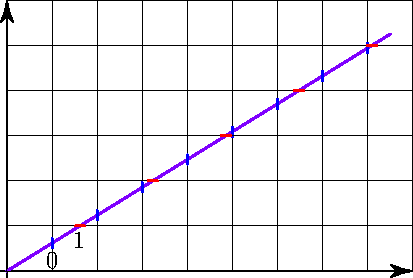
\includegraphics[scale=1.2]{line1}\caption*{$y(x) = \psi x,\ \psi = 1/\phi$, $\phi = (1 + \sqrt{5})/2$ \\ $\Phi_5 = 0100101001001$}
\end{center}
\end{figure}




\end{itemize}



\end{frame}








\begin{frame}{Some Properties of the Fibonacci Word}

\begin{itemize}

\item The factors 11 and 000 are absent in $\Phi$

\item The last two letters of a Fibonacci word are alternately 01 and 10

\item The $n$th digit of $\Phi$ is $$2+\left\lfloor n\varphi\right\rfloor -\left\lfloor \left(n+1\right)\varphi\right\rfloor, $$ where $\phi = (1 + \sqrt{5})/2$ is the golden rartio

\end{itemize}

\end{frame}


















\begin{frame}{The Fibonacci Word and Quasi-Quasicrystals}

Cut-and-projection method gives 

\begin{figure}[!h]
\begin{center}
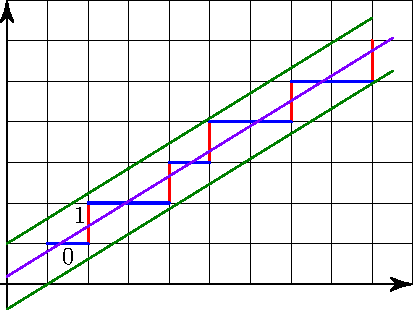
\includegraphics[scale=1.25]{line2}\caption*{$y(x) = \psi x + \frac{1-\psi}{2},\ \psi = 1/\phi$, $\phi = (1 + \sqrt{5})/2$}
\end{center}
\end{figure}


\end{frame}












\begin{frame}{Balanced Words}

\begin{defi}
An infinity word $w$ in the alphabet $\{a, b\}$ is called \emph{balanced} if for any two factors $u$ and $v$ of the same length $n$ $$||u|_{a} - |v|_{a}| \leqslant 1$$ where $|-|_a$ denotes the number of letters $a$ (the Hamming weight). 
\end{defi}

\begin{itemize}

\item The Fibonacci word is an example of balanced word $$\Phi = 01001010010010100101001001010010010100...$$

\item For the Thue-Morse word, however, it is not the case: see, e. g., 00 and 11 $$T = 01101001100101101001011001101001...$$  

\end{itemize}


\end{frame}











\begin{frame}{Geometric Words}

\begin{defi}
An infinite word in two-letter alphabet is called \emph{geometric} if it encodes intersections of a fixed line $y = \alpha x + \rho$ with vertical and horizontal lines of integer lattice 
\end{defi}

\begin{itemize}

\item If $\alpha$ is rational the dynamics is periodic

\item If $\alpha$ is irrational the one is qusi-periodic 

\end{itemize}

\end{frame}






















\begin{frame}{Sturmian Words are Geometric}


\begin{coroll}

For an infinite word in 2-letter alphabet the following conditions are equivalent

\begin{itemize}

\item $f_w(n) = n + 1$

\item $w$ is aperiodic and balanced

\end{itemize}
\end{coroll}

\end{frame}











\begin{frame}

\frametitle{Markov's Result}

\begin{thm}[A. A. Markov, 1882]
Let $\alpha = [0; a_1, a_2, ...]$ be the continued fraction expansion, $\alpha\in (0, 1)$. Then the word $S(\alpha)$ encoded by a line $y = \alpha x$ can be written as follows $$S(\alpha) = \lim\limits_{k} S_k(\alpha)$$ where $$S_k = S_{k-1}^{a_k}S_{k-2}$$ with the initial conditions $S_{-1} = b$ и $S_0 = a$. The letters $a$ and $b$ correspond to vertical and horizontal intersections respectively  
\end{thm}

For the word length sequence $\{ |S_k| \}$ we have $|S_{-1}| = 1$, $|S_0| = 1$ and $$|S_k| = a_k|S_{k-1}| + |S_{k-2}|$$

\end{frame}
















\begin{frame}

\frametitle{Markov's Result}

\begin{block}{Example}

\begin{itemize}
\item Consider the line $y = \psi x$ where $\psi = 1/\varphi$, $\varphi = (1 + \sqrt{5})/2$

 $$\psi = \cfrac{1}{1+\cfrac{1}{1+\cfrac{1}{1+...}}}$$

\item In this case, $S_n = S_{n-1}S_{n-2}$ --- the Fibonacci word
\end{itemize}

\end{block}

\end{frame}















\begin{frame}{Tilings}

\begin{definition}

A simple tiling of $\mathbb{R}^d$:

\begin{itemize}

\item There are only a finite number of tile types, up to translation

\item Each tile is a polytope

\item Tiles meet full-facet to full-facet

\end{itemize}

\end{definition}

\begin{figure}[!h]
\begin{center}
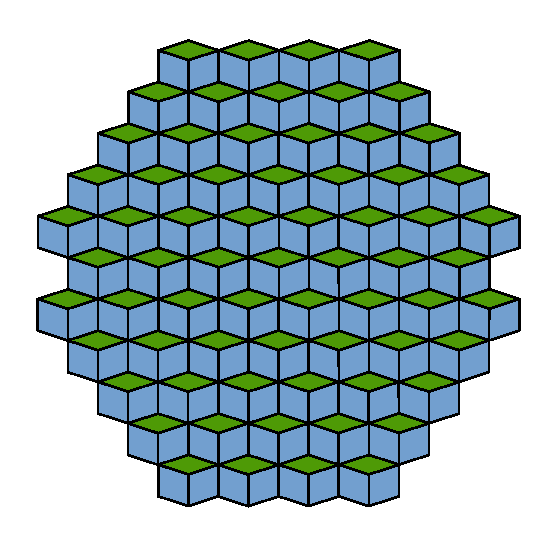
\includegraphics[scale=0.45]{regular_rombs}
\end{center}
\end{figure}



\end{frame}















\begin{frame}{The $\epsilon$-closeness}

\begin{definition}
We say that tilings $T_1$ and $T_2$ are $\epsilon$-close if they are agree on a ball of radius $1/\epsilon$ around the origin, up to translation of size $\epsilon$ or less
\end{definition}

\begin{figure}[!h]
\begin{center}
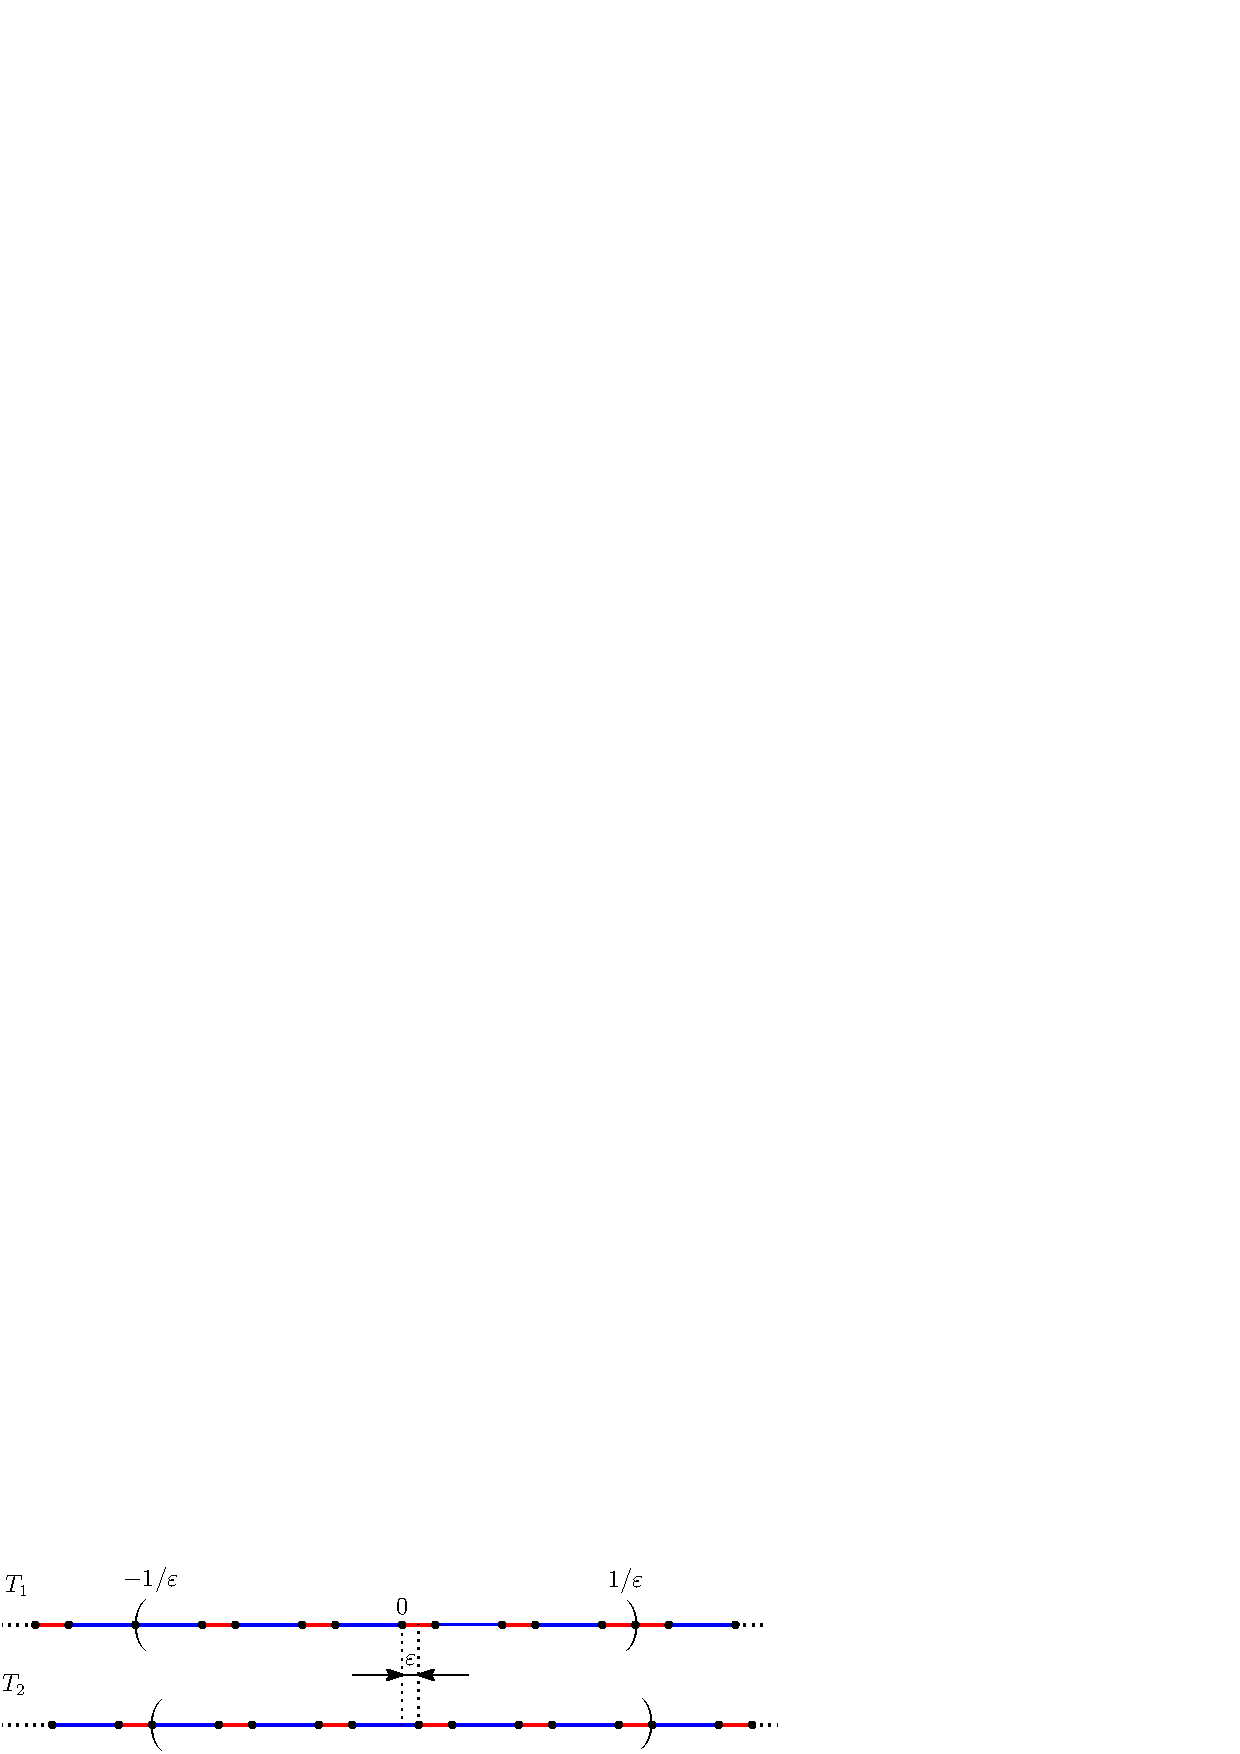
\includegraphics[scale=0.9]{epsilon_closure}
\end{center}
\end{figure}


\end{frame}









\begin{frame}{Tiling Spaces}

\begin{definition}

\begin{itemize}

\item The \emph{orbit} of a tiling $T$ is the set $\Oo(T) := \{T-x\ | \ x\in\mathbb{R}^d\}$ of translates of $T$

\item A \emph{tiling space $\Omega$} is a set that is closed under translation, and complete in the tiling metric 

\item The \emph{hull $\Omega_T$} of a tiling $T$ is the closure of $\Oo(T)$ with respect to the $\epsilon$-closure property

\end{itemize}

\end{definition}


\end{frame}













\begin{frame}{Tiling Spaces}

\begin{block}{Example}

\begin{itemize}

\item Consider a simple 1-dimensional tilling $T_0$ with just one kind of tile. Suppose its length is 1 and its color is blue

\item Obviously, $T_0 = T_0 - 1$. So, $\Omega_{T_0}$ is a circle

\begin{figure}[!h]
\begin{center}
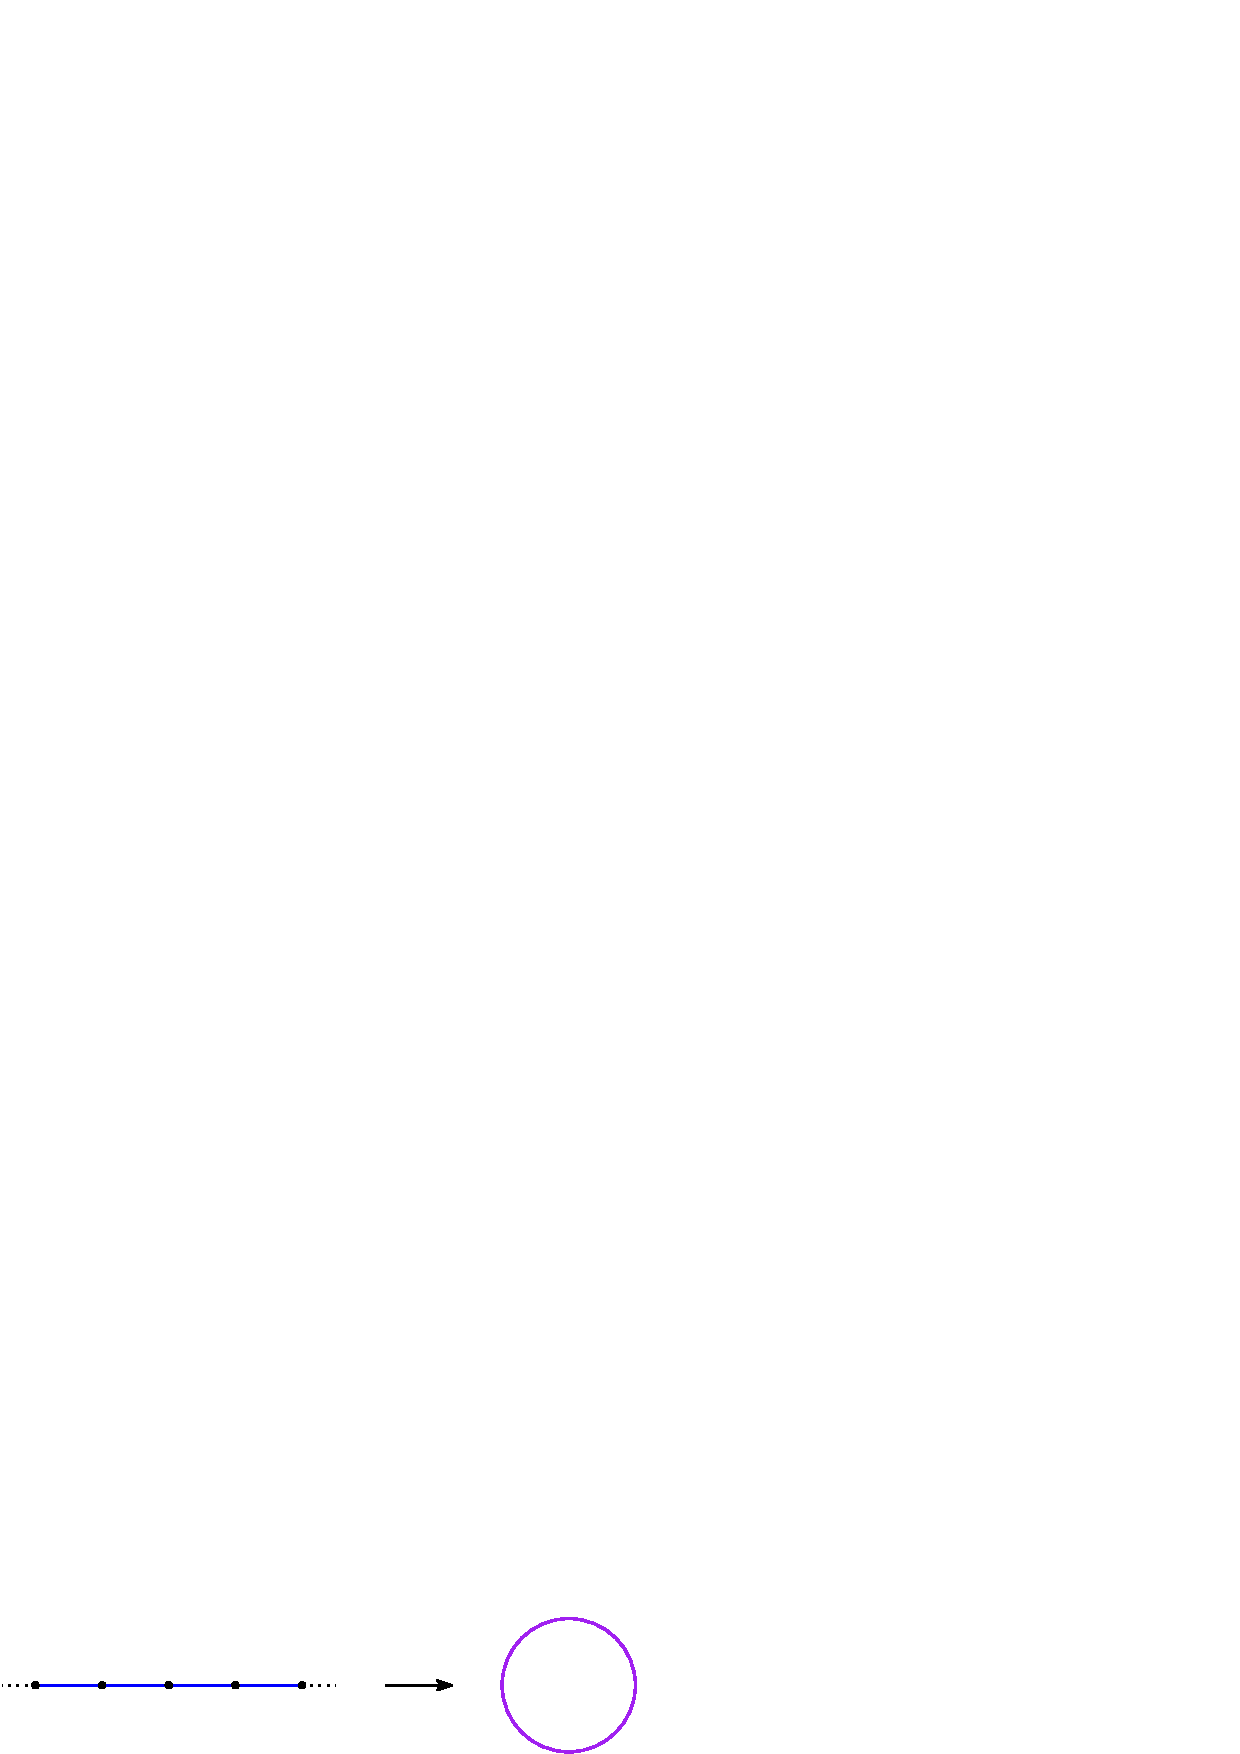
\includegraphics[scale=1]{T0}
\end{center}
\end{figure}

\end{itemize}

\end{block}

\end{frame}













\begin{frame}{Tiling Spaces}

\begin{block}{Example}

\begin{itemize}

\item Consider an 1-dimensional tilling $T_1$ with one red tile of length 2 and other blue tiles of length 1

\item Any tiling with one red tile is in $\Oo(T_1)$, and hence in $\Omega_{T_1}$

\item Tilings with no red tiles are also in $\Omega_{T_1}$ by simple reasons

\item So, $\Omega_{T_1}$ looks like the circle $\Omega_{T_0}$ and the line $\Oo(T_1)$ with both ends of the line asymptotically approaching the circle 

\end{itemize}

\begin{figure}[!h]
\begin{center}
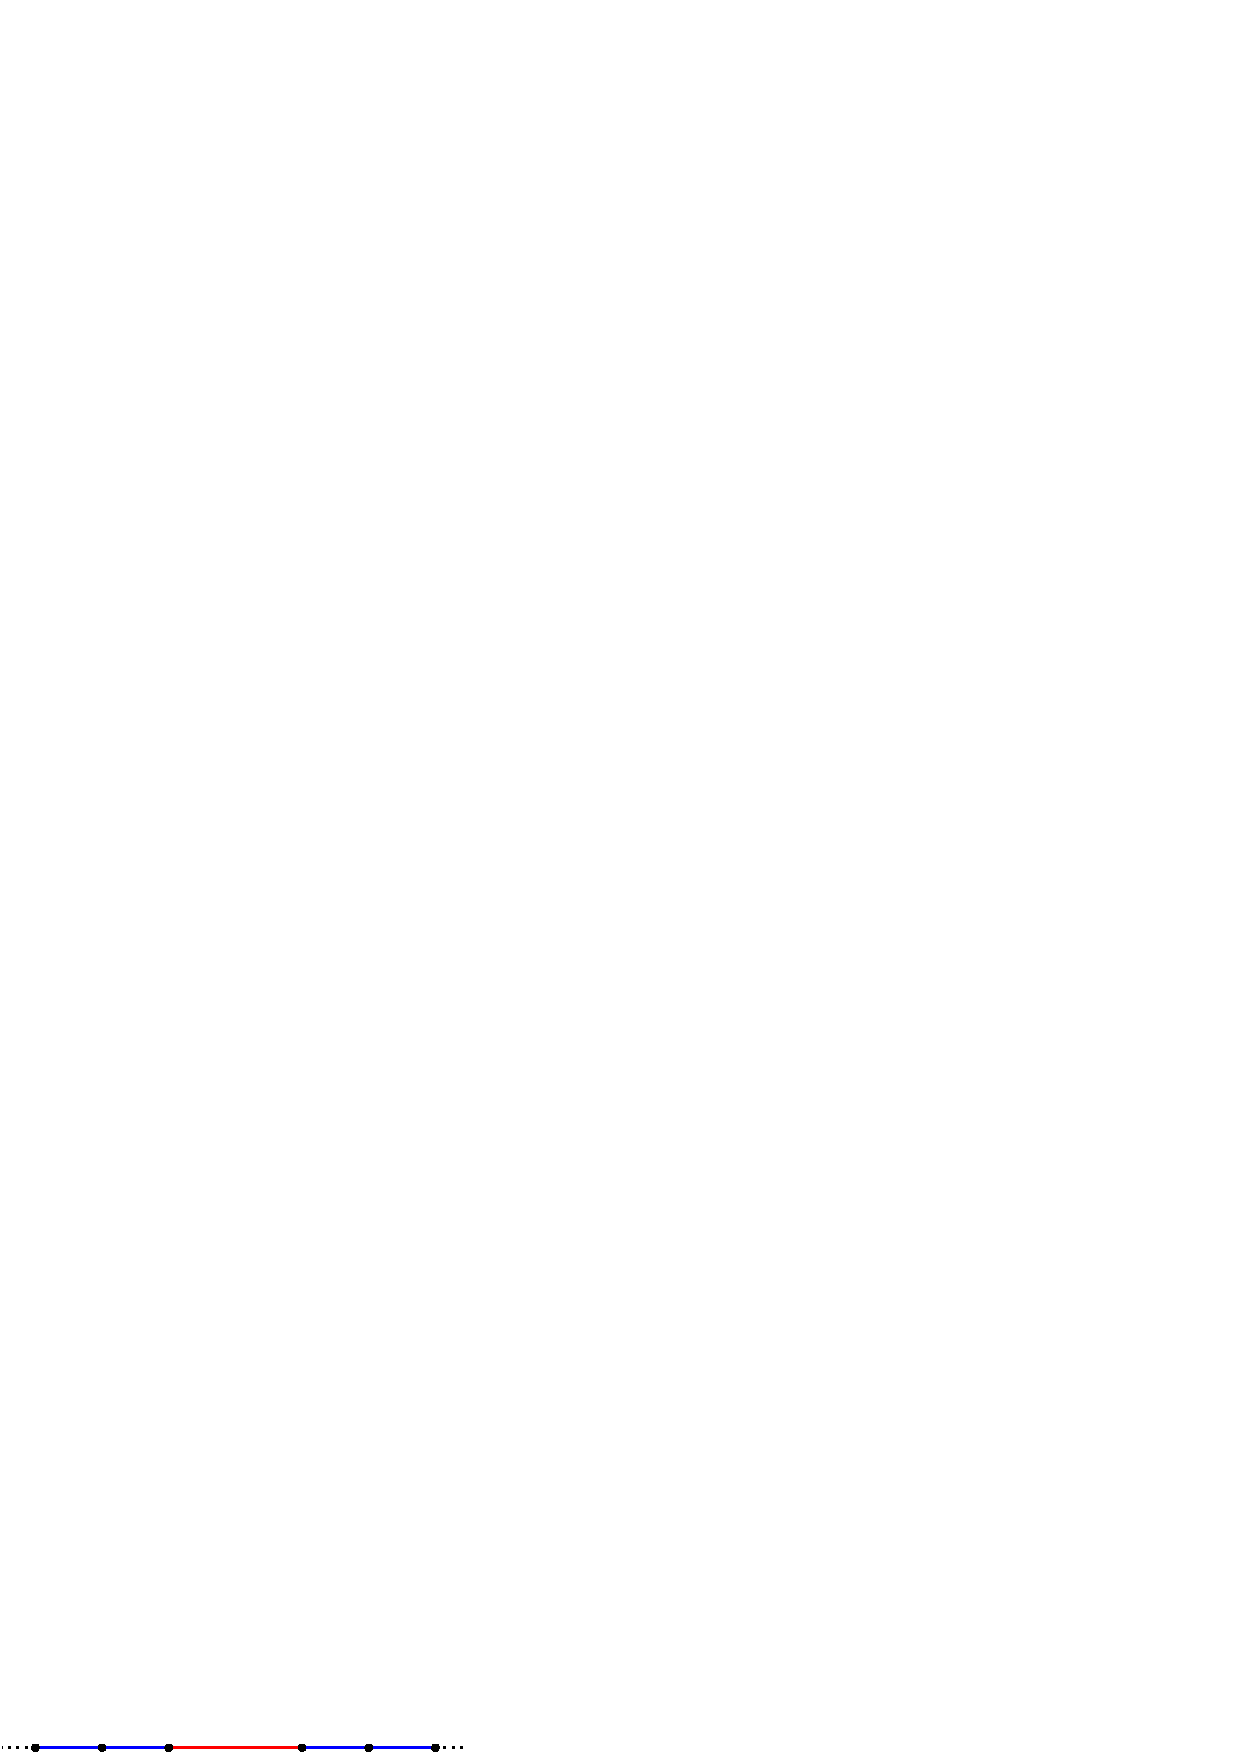
\includegraphics[scale=1]{T1}
\end{center}
\end{figure}

\end{block}

\end{frame}














\begin{frame}{Tiling Spaces}

\begin{block}

\begin{figure}[!h]
\begin{center}
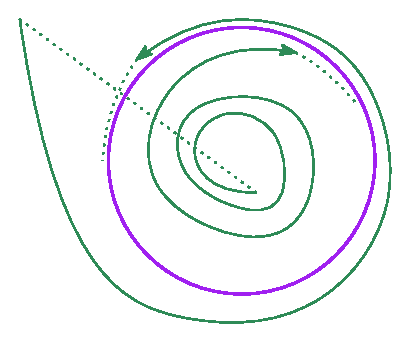
\includegraphics[scale=1]{solenoid}
\end{center}
\end{figure}

\end{block}


\end{frame}


















\begin{frame}{Tiling Spaces}

\begin{theorem}
If $T$ is a simple tiling then $\Omega_T$ is compact
\end{theorem}

\begin{itemize}

\item For a tiling $T$ one can approximate the space $\Omega_T$ via CW complexes $\Gamma_n$ from the \emph{Gähler's construction}

\item There is a sequence of forgetful maps $f_n: \Gamma_{n+1}\to\Gamma_n$. The space $\Gamma_{n}$ knows about surrounding $n$ layers in some sence

\item Hence, one can form an inverse limit and it will homeomorphic to $\Omega_T$ $$\Omega_T = \underleftarrow{\lim} \, \Gamma_n$$  

\item In the case of substitution tilings, it is more convenient to use the \emph{Anderson-Putnam construction} of $\Gamma_n's$


\end{itemize}

\end{frame}


















\begin{frame}{Topological Invariants of Tiling Spaces}

\begin{itemize}

\item $\Omega_T$ has one connected component, but uncountably many path-component

\item Each path component in a tiling space is an orbit under $\mathbb{R}^d$. Such an orbit of an aperiodic tiling is contractible, so $\pi_n(\Omega_T) = 0$ and $H_n(\Omega_n; A) = 0$ for $n > 0$, $A$ is abelian

\item Čech cohomology does better

 $$\check{H}^\ast\left ( \underleftarrow{\lim} \, \Gamma_n \right ) \cong \underrightarrow{\lim} \, \check{H}^\ast (\Gamma_n) \cong  \underrightarrow{\lim}\, H^\ast(\Gamma_n)$$
 
\begin{block}{Example}
$\check{H}^1$ of the Fibonacci tiling space is $\mathbb{Z}\oplus\phi\mathbb{Z}$, $\phi = (1 + \sqrt{5})/2$
\end{block}

\end{itemize}

\end{frame}












\begin{frame}{Prodefinition of $n$-valued Groups}

\begin{block}{Prodefinition}
A \emph{hypergroup} is a promonoidal category structure on a discrete poset $X$, whose promultiplication $X\times X\to \EuScript{G}(X)$ takes values in the 2-category of non-empty groupoids, with some additional groupal properties  
\end{block}


Recall, a promonoidal category is a category $\EuScript{C}$ together with 

\begin{itemize}

\item A profunctor (promultiplication) $\EuScript{C}\times\EuScript{C}\pto \EuScript{C}$

\item A profunctor (prounit) $J : 1 \pto \EuScript{C}$

\item Associativity $P\circ (P\times 1)\cong P\circ (1\times P)$

\item Unit isomorphisms $P\circ (J\times 1)\cong 1$, and $P\circ (1\times J)\cong 1$ 

\end{itemize} 

A fancy arrow $A\pto B$ means a functor $B^{\mathrm{op}}\times A\to \mathrm{Set}$. The composition of $F: A\pto B$ and $G: B\pto C$ is defined to be $$(G\circ F)(c, a) = \int \limits^{a\in A} F(b, a)\otimes G(c, b)$$

\end{frame}












\begin{frame}{Symmetric Powers of a Space}
\begin{itemize}

\item For a topological space $X$, let $(X)^n$ denote its $n$-fold
symmetric power, i. e., $(X)^n=X^n/\Sigma_n$ where the symmetric group $\Sigma_n$ acts by permuting the coordinates


\item An element of $(X)^n$ is called an $n$-subset of $X$ or just an $n$-set. It is a subset with multiplicities of total cardinality $n$


\begin{block}{Example}
The spaces $(\mathbb{C})^n=\mathbb{C}^n/\Sigma_n$
and $\mathbb{C}^n$ are identified using the map $\mathcal{S}:\mathbb{C}^n\to\mathbb{C}^n$
whose components are given by
\[
(z_1,z_2,\dots,z_n)\to \sigma_r(z_1,z_2,\dots,z_n),\; 1\leqslant r\leqslant n,
\]
where $\sigma_r$ is the $r$-th elementary symmetric polynomial
\end{block}


\end{itemize}
\end{frame}
















\begin{frame}{$n$-valued Group Structure}
An \emph{$n$-valued multiplication} on $X$ is a map
\[
\mu: X\times X \to (X)^n\,:\,\mu(x,y)=x*y=[z_1,z_2,\dots, z_n], \; z_k=(x*y)_k
\]

\begin{itemize}

\item \emph{Associativity.} The $n^2$-sets
\begin{gather*}[x*(y*z)_1,x*(y*z)_2,\dots,x*(y*z)_n],\\
[(x*y)_1*z,(x*y)_2*z,\dots,(x*y)_n*z]
\end{gather*}
are equal for all $x,y,z\in X$


\item \emph{Unit.} $e\in X$ such that $e*x=x*e=[x,x,\dots,x]$\; for all\; $x\in X$

\item \emph{Inverse.} A map $\mathrm{inv}\colon X\to X$ such that

\[
e\in \mathrm{inv}(x)* x\text{ and }\; e \in x*\mathrm{inv}(x)\text{ for all }x\in X
\]

\begin{block}

The map $\mu$ defines an $n$-valued group structure on $X$ \\
if it is associative, has a unit and an inverse

\end{block}

\end{itemize}
\end{frame}














\begin{frame}{Example: $2$-valued Group Structure on $\mathbb{Z}_{+}$}

\begin{itemize}

\item Consider the semigroup of nonnegative integers $\mathbb{Z}_+$

\item Define the multiplication $\mu\colon \mathbb{Z}_+\times \mathbb{Z}_+\to (\mathbb{Z}_+)^2$
by the formula $x*y=[x+y,|x-y|]$

\item \emph{The unit:} $e=0$

\item \emph{The inverse:} $\mathrm{inv}(x)=x$.

\item \emph{The associativity:} one has to verify that the $4$-subsets of $\mathbb{Z}_+$
\[[x+y+z, |x-y-z|,x+|y-z|, |x-|y-z||]\]
and
\[[x+y+z,|x+y-z|,|x-y|+z,||x-y|-z|]\]
are equal for all nonnegative integers $x,y,z$

\end{itemize}

\end{frame}

















\begin{frame}{Example: $n$-valued Group Structure on $\mathbb{C}$}

\begin{itemize}

\item Define the multiplication $\mu\colon \mathbb{C}\times \mathbb{C}\to \mathbb{(C)}^n$
by the formula

\[
x*y=[(\sqrt[n]{x}+\varepsilon^r \sqrt[n]{y}\,)^n,\quad 1\leqslant r\leqslant n],
\]
where $\varepsilon \in \mathbb{Z}_n$ is a primitive $n$th root of unity

\item \emph{The unit:} $e=0$

\item \emph{The inverse:} $\mathrm{inv}(x)=(-1)^n x$


\item The multiplication is described by the polynomial equations


\[
p_n(x,y,z)=\prod_{k=1}^n\big(z-(x*y)_k\big) = 0
\]
For instance,

\[
p_1=z-x-y,\quad p_2=(z+x+y)^2-4(x y+y z+z x),
\]
\[
p_3=(z-x-y)^3-27xyz
\]
\end{itemize}

\end{frame}














\begin{frame}{Homomorphisms of $n$-valued Groups}


\begin{defi}
A map $f: X\to Y$ is called \emph{a homomorphism of $n$-valued groups} if 

\begin{itemize}

\item $f(e_X)=e_Y$

\item $f(\mathrm{inv}_X(x))=\mathrm{inv}_Y(f(x))$ for all $x\in X$

\item $\mu_{Y}(f(x),f(y))=(f)^n\mu_X(x,y)$ for all $x, y\in X$

\end{itemize}

\end{defi}

So, the class of all $n$-valued groups forms a category \bf{MultValGrp}


\end{frame}















\begin{frame}{Reducible $n$-valued Groups}

\begin{itemize}

\item For each $m\in\mathbb{N}$, an $n$-valued group on $X$, with some multiplication $\mu$, can be regarded as an $mn$-valued group by using as the multiplication the composition


\[
X\times X\overset{\mu}\longrightarrow(X)^n\overset{(D)^m}{\longrightarrow} (X)^{m n},\;\text{ where } D\text{ is diagonal}
\]

\begin{defi}
An $n$-valued group on $X$ is called \emph{reducible} if there is an isomorphism $f:X\to Y$ where $Y$ is an $n$-valued group with a multiplication $\mu_n = \mu_k^m$, $n = mk$
\end{defi}

\end{itemize}

\end{frame}















\begin{frame}{Kernels and Images}

\begin{lemm}
Let $f: X\to Y$ be a homomorphism of $n$-valued groups. Then
 
\begin{itemize}

\item $\ker(f)=\{x\in X\mid f(x)=e_Y\}$ is an $n$-valued group

\item $f(x_1) = f(x_2)\Leftrightarrow (f)^n(zx_1) = (f)^n(zx_2)$ for all $z \in \ker(f)$

\item Suppose that the map $\mathrm{inv}: X\to X$ is uniquely defined. Then $\ker(f) = \{e\}$ if and only if any equality $f(x_1) = f(x_2)$ implies $x_1 = x_2$ 

\item $\mathrm{Im} (f)=\{y\in Y\mid y=f(x), x\in X\}$ is an $n$-valued group

\end{itemize}
\end{lemm}
\end{frame}






























\begin{frame}{Coset Groups}

\begin{itemize}

\item Let $G$ be a (1-valued) group with the multiplication $\mu_0$, the unit $e_G$, and $\mathrm{inv}_G(u) = u^{-1}$

\item Let $A\hookrightarrow \mathrm{Aut} G$ be a finite group of order $n$ 

\item Denote by $X$ the quotient space $G/A$ of $G$, and denote by $\pi : G\to X$ the quotient map

\item Define the $n$-valued multiplication $\mu : X\times X\to (X)^n$ by the formula
\[
\mu(x,y)=[\pi(\mu_0(u,v^{a}))\ | \ a\in A]
\]
where $u\in \pi^{-1}(x), \ v\in \pi^{-1}(y)$ and $v^a$\, is the image of the action of $a \in A$ on $v\in G$

\end{itemize}

\begin{thm}
The multiplication $\mu$ defines some $n$-valued coset group structure $(G, A)$ with the unit $e_X = \pi(e_G)$ and the non-ambiguity defined map $\mathrm{inv}(u) = \pi(u^{-1})$ where $\pi(u) = x$
\end{thm}

\end{frame}


















\begin{frame}{Coset Groups}

\begin{block}{Example}

\begin{itemize}

\item Consider $G=\{a,b\mid a^2=b^2=e\}$

\item The interchange of $a$ and $b$ is an element of order 2 of $\mathrm{Aut} G$

\item Then we have on the set $X = G/A = \{ u_{2n}, u_{2n + 1} \}$, $n\geqslant 0$ where

$$u_{2n} = [(ab)^n, (ba)^n], \ u_{2n+1} = [a(ba)^n, b(ab)^n]$$ 

\item The multiplication: $$ u_k*u_{\ell}=[u_{k+\ell},u_{| k-\ell |}]$$

\item Thus, $X$ is isomorphic to the $2$-valued group on $\mathbb{Z}_+$ constructed above

\end{itemize}

\end{block}

\end{frame}


















\begin{frame}{$n$-valued Dynamics}

\begin{itemize}

\begin{defi}
An \emph{\it $n$-valued dynamics} $T$ on a space $Y$ is a map $T : Y \to (Y)^n$
\end{defi}

\item If $Y$ is a state space then the $n$-valued dynamics $T$ defines possible states $T(y) = [y_1,\ldots, y_n]$ at the moment $(t+1)$ as a state function of $y$ at the moment $t$

\end{itemize}

\begin{block}{Example}

\begin{enumerate}

\item Consider $F(x,y) = b_0(x)y^n + b_1(x)y^{n-1} + \cdots + b_n(x),\; x,y\in \mathbb{C}$.

\item The equation $F(x,y)=0$ defines an $n$-valued dynamics
\[
T\colon \mathbb{C}\to (\mathbb{C})^n \;:\; T(x) = [y_1,\dots, y_n]
\]
where $[y_1,\dots, y_n]$ --- $n$-set of roots of $F(x,y)=0$

\end{enumerate}

\end{block}


\end{frame}













\begin{frame}{$n$-valued Growth Function}

\begin{itemize}

\item Let $T\colon Y \to (Y)^n$ be an $n$-valued dynamics. For any $y\in Y$ define the $n$-valued growth function $\xi_y\colon \mathbb{N}\to \mathbb{N}$ where $\xi_y(k)$ --- the number of different points in the set $T^k(y)$

\begin{block}{Problem}
Characterize such $n$-valued dynamics $T$ that functions $\xi_y(k)$ have polynomial growth for any $y\in Y$
\end{block}

\begin{figure}
\centering
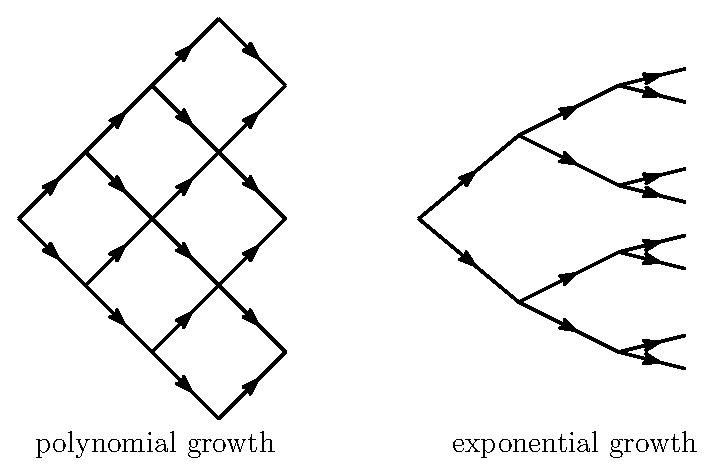
\includegraphics[width=0.6\linewidth]{grid_and_tree}
\end{figure}

\end{itemize}

\end{frame}


















\begin{frame}{$n$-valued Actions}

An action of $n$-valued group $X$ on a space $Y$ is defined by the map
\[
\varphi\colon X\times Y\to (Y)^n\;:\; \varphi(x,y) = x\cdot y = [y_1,\ldots,y_n]
\]
such that

\begin{itemize}

\item for any $x_1,x_2\in X$ and $y\in Y$ the following $n^2$-sets coincide:
\[
x_1\cdot(x_2\cdot y) = [x_1\cdot y_1,\ldots,x_1\cdot y_n] \text{ and }(x_1 x_2)\cdot y = [z_1\cdot y,\ldots,z_n\cdot y]
\]
where $x_2\cdot y = [y_1,\ldots,y_n]$\; и\; $x_1 x_2 = [z_1,\ldots,z_n]$

\item $e\cdot y = [y,\ldots,y]$ for any $y\in Y$

\end{itemize}

\end{frame}














\begin{frame}{$n$-valued Cyclic Dynamics}

\begin{defi}
An $n$-valued group $X := \langle x \rangle$ is called \emph{cyclic} if it is generated by the only element $x\in X$
\end{defi}

\begin{defi}
Consider $n$-valued dynamics $T\colon Y \to (Y)^n$ with $X = \langle a\rangle$. The generator $a$ is called the \emph{generator of the cyclic dynamics $T$}
\end{defi}

\begin{thm}[A. A. Gaifullin, P. V. Yagodovskii, 2007]
An $n$-valued dynamics $T$ has a generator $a\in X$ if and only if there exists such a dynamics $T^{-1}\colon Y \to (Y)^n$ that for any $y_1$, $y_2\in Y$ the multiplicity of $y_2$ in $T(y_1)$ equals the multiplicity of $y_1$ in $T^{-1}(y_2)$
\end{thm}

\end{frame}













\begin{frame}{$n$-valued Cyclic Group Growth Problem}

\begin{itemize}

\item Let $X = \langle a\rangle$ be a cyclic $n$-valued group

\item Then there is the left action of $X$ on itself $$T : X \to (X)^n, \ T(x) = a\cdot x$$

\item Recall $\xi_a(k)$ is a number of different elements in $T^k(a)$

\begin{block}{Notation}

Denote by $\mathbb{G}_\phi(G)$ the $n$-valued group obtained from the construction above for some ordinary group $G$ and some automorphism group element $\phi$ 

\end{block}


\end{itemize}

\end{frame}








\begin{frame}{The Case of $\mathbb{Z}/3\ast\mathbb{Z}/3$ with $\mathbb{Z}/2<\mathrm{Aut}$}

\begin{prop}\label{z3z3}
For the group $\mathbb{Z}/3\ast\mathbb{Z}/3 = \langle a, b\ | \ a^3=b^3=1 \rangle$ and the automorphism $\varphi:$ $a\mapsto b$ the corresponding 2-valued group $\mathbb{G}_\varphi\left(\mathbb{Z}/3\ast\mathbb{Z}/3\right)$ has the growth function $$\xi_{[a, b]}(k) = F_{k+3} - 1 =  \cfrac{1}{\sqrt{5}}\left ( \left(\cfrac{1 + \sqrt{5}}{2} \right)^{k+3} - \left( \cfrac{1-\sqrt{5}}{2} \right )^{k+3} \right ) - 1.$$ In particular, the growth is exponential: $$\xi_{[a, b]}(k) \sim \cfrac{\varphi^{k+3}}{\sqrt{5}}$$ where $k\to\infty$ and $\varphi = (1+\sqrt{5})/2$. 
\end{prop}

\end{frame}




\begin{frame}{$n$-bonacci Sequence}

\begin{defi}
The $n$-bonacci sequence $\{F_k^{(n)}\}$ is defined recursively as follows: $$F_k^{(n)} = F_{k-1}^{(n)} + ... + F_{k-n}^{(n)},$$ initial conditions are $F_0 = ... = F_{n-2} = 0\text{ и } F_{n-1} = 1.$
\end{defi}

\begin{block}{Example}
Fibonacci sequence: $$0, 1, 1, 2, 3, 5, 8, 13, 21, ... $$
Tribonacci sequence: $$0, 0, 1, 1, 2, 4, 7, 13, 24, ... $$ 
\end{block}

\end{frame}





\begin{frame}{The Case of $\mathbb{Z}/m\ast\mathbb{Z}/m$ with $\mathbb{Z}/2<\mathrm{Aut}$}

\begin{prop}
The number $S_k$ of new words, appearing on the step $k$, equals $$S_k = F^{(m-1)}_{k+m-2}$$ when $k\geqslant -(m-2)$. 
\end{prop}

\end{frame}
















\begin{frame}{The Case of $\mathbb{Z}/m\ast\mathbb{Z}/m$ with $\mathbb{Z}/2<\mathrm{Aut}$}

\begin{prop}[M. K.]
For the group $\mathbb{Z}/m\ast\mathbb{Z}/m = \langle a, b\ | \ a^m = b^m = 1 \rangle$, $m\geqslant 3$ with the automorphim $\varphi: a\mapsto b$ we have $$\xi_{[a, b]}(k)\sim\frac{r^{k+1}}{mr-2(m-1)}$$ where $k\to\infty$ and $r$ is the positive root of the polinomial $\chi(\lambda) = \lambda^n - \lambda^{n-1} - ... - 1$. In particular, $\mathbb{G}_\varphi(\mathbb{Z}/m\ast\mathbb{Z}/m)$ has the polinomial growth if and only if $m = 2$
\end{prop}



\end{frame}








\begin{frame}{The Case of $\left ( \mathbb{Z}/2\right )^{\ast s}$ with $\mathbb{Z}/s<\mathrm{Aut}$}

\begin{prop}
For the group $\left ( \mathbb{Z}/2\right )^{\ast s}= \langle a_1, ..., a_s \ | \ a_1^2=...=a_s^2=1 \rangle$ with the automorphism $a_i\mapsto a_{i+1}$ $($indices move modulo $s)$ we have the $s$-valued group with the growth $$\xi_{[a_1, ..., a_s ]}(k)=\begin{cases}
\dfrac{\left(s-1\right)^{k}-1}{s-2}+1, & s\geqslant3\\
k + 1, & s=2
\end{cases}$$ In particular, the growth is polynomial if and only if $s = 2$  

\end{prop}

\end{frame}








\begin{frame}{$\mathbb{Z}/3\ast\mathbb{Z}/3$ and Symbolic Dynamics}


\begin{figure}[!h]
\begin{center}
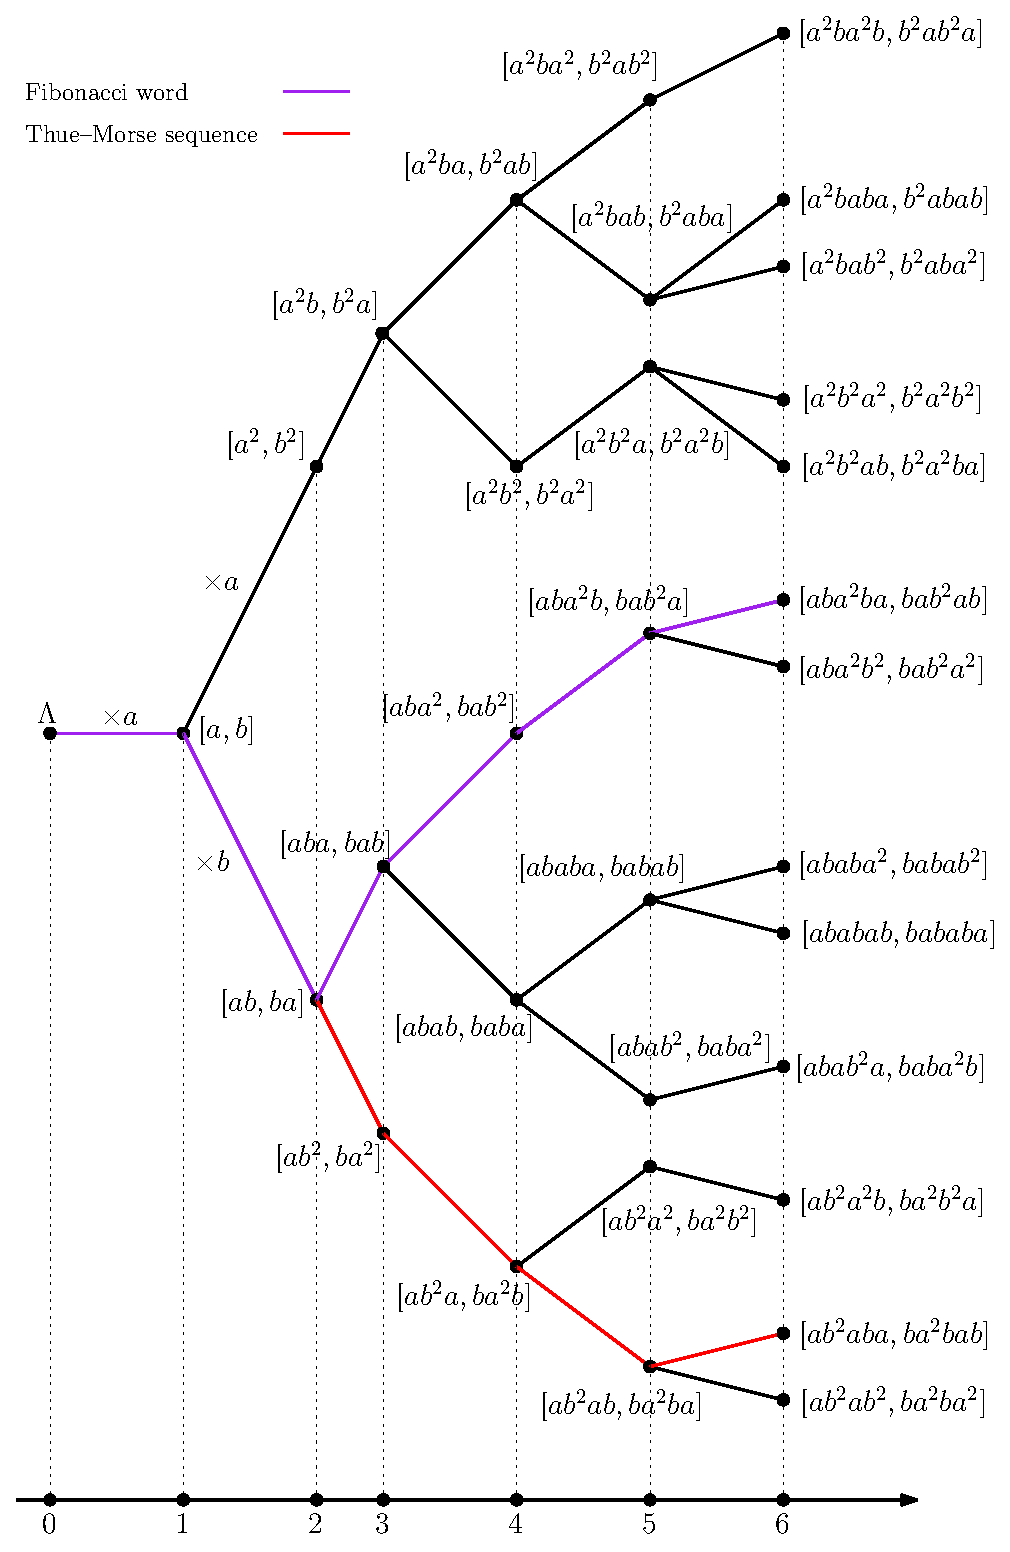
\includegraphics[scale=0.3]{tree}
\end{center}
\end{figure}

\end{frame}

















\begin{frame}{$\mathbb{Z}/3\ast\mathbb{Z}/3$ and Symbolic Dynamics}


An algorithm construction of a directed tree $\Gamma$, as vertices having the elements of 2-valued group $\mathbb{G}$:

\begin{enumerate}[\bf 1]

\setcounter{enumi}{-1}

\item We start with the vertex, corresponding to the empty set $\Lambda$ --- the root of our tree

\item Add the vertex $[a, b]$ adjacent to the root

\item Add two edges to the last vertex: each of them corresponds to an addition a letter ($a$ or $b$) on the right hand side. Now we have two words of length 2:  $[a^2, b^2]$ and $[ab, ba]$

\end{enumerate}

\end{frame}






\begin{frame}{$\mathbb{Z}/3\ast\mathbb{Z}/3$ and Symbolic Dynamics}

\begin{defi}
We say that a word is \emph{cube-free} (it doesn't agree with the common use) if any word in the (natural) normal form of the group $\mathbb{Z}/3\ast\mathbb{Z}/3 = \langle a, b\ | \ a^3=b^3=1 \rangle$
\end{defi}

\begin{enumerate}[\bf 1]

\setcounter{enumi}{3}

\item On the step $k$ we start with all cube-free words of length $k-1$ and add for each vertex 1 or 2 edges according to the principle:

\begin{itemize}

\item If a word ends with the first power of a letter then we will add 2 edges, corresponding to the multiplications with $a$ and $b$

\item If a word ends with the square of a letter then we will add exactly one edge, corresponding to the remaining letter 

\item The edge, corresponding to the multiplication with $a$, lies higher than the other one 
 
 \end{itemize}

\end{enumerate}

\end{frame}










\begin{frame}{Properties of $\Gamma$}



\begin{itemize}

\item On the level $k$ of the tree $\Gamma$ top down, all cube-free words of length $k$ place in lexicographic ascending order and their number is $F_{k+1}$. Using the binary notation $a\leftrightarrow 0$, $b\leftrightarrow 1$, this order coincides with the natural order on the binary numbers 

\item If one picts, down to top, the vertex having the number $F_k$ on each $k$-level of $\Gamma$ then the resulting vertex sequence will form the route $ab(aab)$ in $\Gamma$ 


\end{itemize}



\end{frame}





\begin{frame}{Properties of $\Gamma$}


\begin{figure}[!h]
\begin{center}
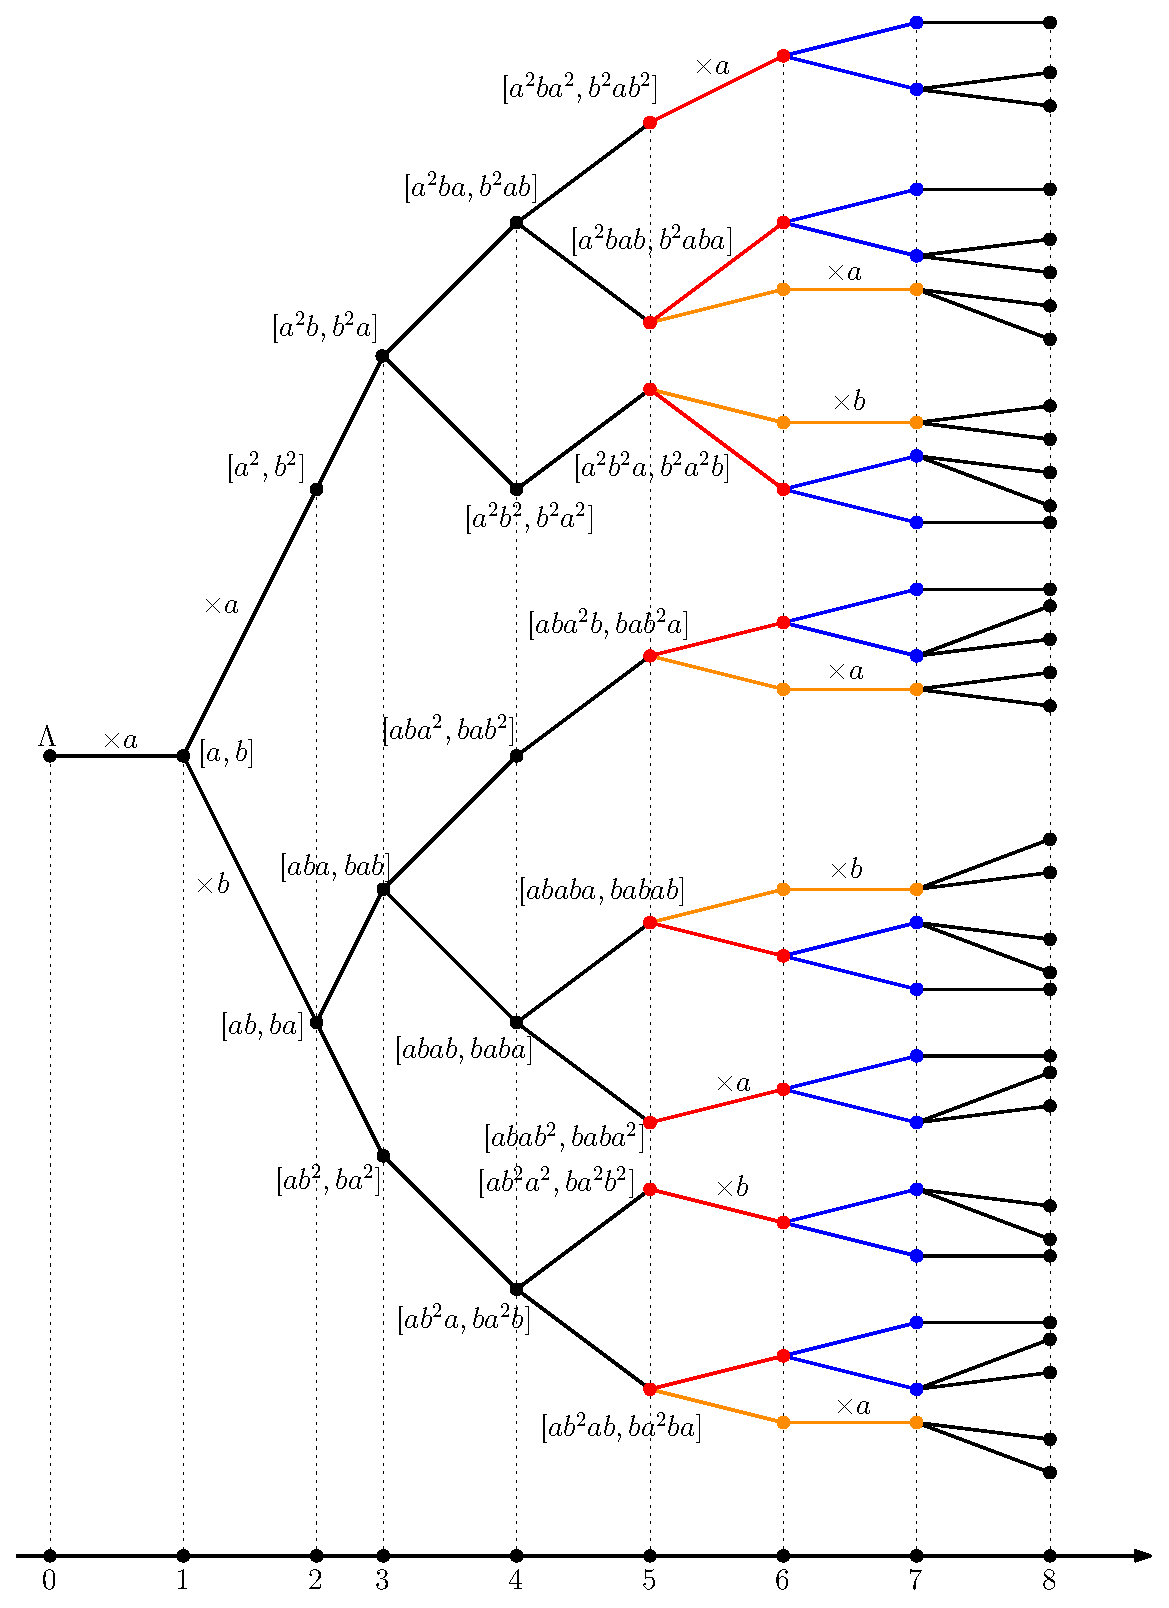
\includegraphics[scale=0.3]{tree2}
\end{center}
\end{figure}

\end{frame}











\begin{frame}{Properties of $\Gamma$}

The latter can be formulated more generally in the following


\begin{prop}[M. K.]
For an infinite cube-free word $\Psi$, consider the factor sequence $\{\Theta_k\}$ of the form $$\Psi aabaabaab... = \Psi(aab)$$ $$\Theta_1 = \Psi,\ \Theta_2 = \Psi a,\ \Theta_3 = \Psi aa,\ \Theta_4 = \Psi aab, \ \Theta_5 = \Psi aaba, \ ...$$ where the last letter of pre-period word $\Psi$ differs from $a$. Then the number $Q_k$ of cube-free words satisfies the recursive equality, with words being grater or equal $\Theta_k$ lexicographically: $$Q_k = Q_{k-1} + Q_{k-2}.$$  
\end{prop}


\end{frame}











































\begin{frame}{Properties of $\Gamma$}

\begin{figure}[!h]
\begin{center}
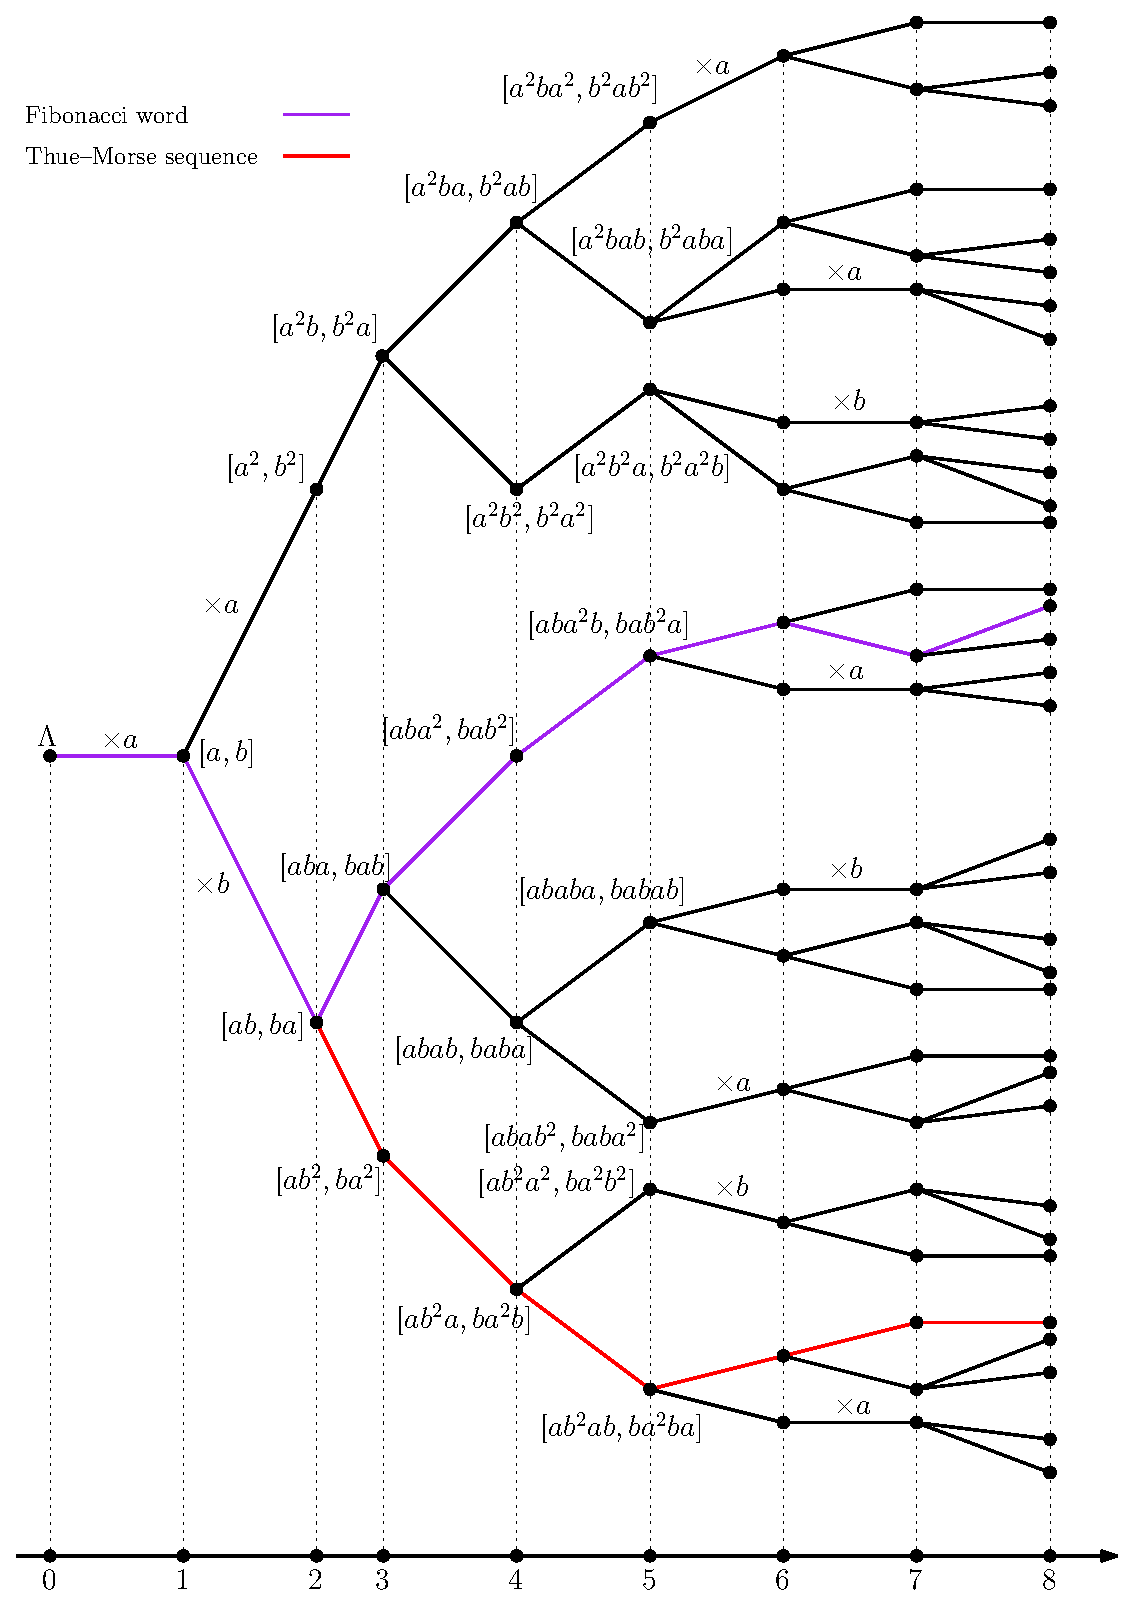
\includegraphics[scale=0.3]{tree3}
\end{center}
\end{figure}

\end{frame}


















\begin{frame}{Conclusion}

\begin{itemize}

\item This construction of the tree might give some fruitful intuition about quasi-periodic words

\item At present, there are gaps in the $n$-valued-group growth study 

\item The items above will be the subjects of further study  

\end{itemize}

\end{frame}



















\begin{frame}

\begin{center}
\Huge \emph{Thank you!}
\end{center}

\end{frame}









\begin{frame}[noframenumbering,plain,allowframebreaks]{References}
    \nocite{*}
\bibliographystyle{plain}
\bibliography{data}

    %\printbibliography[heading=none]
    
    
\end{frame}








\end{document}
